\documentclass[conference]{IEEEtran}
\usepackage{amsmath,amssymb}
\usepackage{graphicx}
\usepackage{booktabs}
\usepackage{cite}
\usepackage{url}

\begin{document}

\title{Probe Before You Trust: Evidence-Bounded GNSS Re-Admission for Spoofing-Resilient Vehicle Navigation}

\author{\IEEEauthorblockN{Pratyaksh Gupta}
\IEEEauthorblockA{School of Computer Science and Engineering\\
Vellore Institute of Technology, Vellore, India}
\and
\IEEEauthorblockN{Padma Priya R}
\IEEEauthorblockA{School of Computer Science and Engineering\\
Vellore Institute of Technology, Vellore, India}}

\maketitle

\begin{abstract}
Most GNSS spoofing defences for vehicles stop at detection: once an alarm fires, the receiver is excluded, and it is let back in as soon as the alarm goes quiet. That last step is the weak point, because an attacker who pauses briefly is welcomed back. We describe FedQPNT, a navigation stack in which a learned detector and a set of physics-based checks drive a continuous trust weight on GNSS, with separate weights for position and for the receiver clock. GNSS is re-admitted only after a ``shadow probe'' in which incoming fixes are tested against the coasted inertial solution without being applied to it. We also add a second-order attitude term to the filter covariance so that this test stays meaningful during long coasts. The design was evaluated in a pre-registered simulation study of 5{,}340 runs on 30 unseen seeds, two IMU grades and fifteen scenario families. FedQPNT raised the alarm about 0.5\,s earlier than a detect-and-exclude baseline (Holm-adjusted $p=0.0037$), cost nothing under nominal driving and jamming, and cut clock error under a displaced meaconer from 5{,}217\,ns to 634\,ns. It was worse than doing nothing against small drift spoofs, and neither a calibrated cold-atom accelerometer nor federated training of the detector gave a measurable benefit. We report these outcomes as measured.
\end{abstract}

\begin{IEEEkeywords}
GNSS spoofing, meaconing, sensor fusion, trust management, Kalman filter, federated learning, atom interferometry
\end{IEEEkeywords}

\section{Introduction}

Satellite navigation reaches a receiver at roughly $-130$\,dBm, well below thermal noise. A cheap transmitter can therefore jam it, and a slightly more capable one can spoof it, producing a believable but false position or time~\cite{psiaki2016gnss,humphreys2008assessing}. Meaconing is a particularly awkward case: the attacker records genuine signals in one place and replays them in another, so every signal looks authentic while both position and clock are shifted.

Inertial sensors are immune to all of this, but they drift. A practical vehicle therefore has to make a running judgement about how much to believe GNSS. Recent work has made good progress on the detection half of that judgement, including federated detectors trained across vehicles~\cite{khan2025enhancing,chai2025navigation,liu2026g2fl}. The other half, deciding \emph{when to believe GNSS again}, has received less attention. In a detect-and-exclude scheme, re-admission is usually memoryless: the moment the detector quietens, GNSS is back. An attacker who switches off for a few seconds, or who drifts slowly enough to stay under the alarm threshold, takes the navigation solution with it.

This paper is about that second half. Our contributions are:
\begin{enumerate}
\item a three-state trust engine (TRUST, DISTRUST, PROBE) that scales GNSS measurement noise continuously and re-admits GNSS only after a shadow consistency test against the coasted state, with a proven bound of 223 trust cycles per hour;
\item separate trust channels for position and clock, with each piece of physical evidence routed to the channel it actually informs;
\item a closed-form second-order attitude term for the error-state filter covariance, without which the re-admission test rejected genuine GNSS after long coasts;
\item a pre-registered evaluation, with code frozen before any test seed was run, that reports both the gains and the cases where the design loses.
\end{enumerate}
The full system also contains a cold-atom interferometer (CAI) model and a federated detector. Both are evaluated here, but neither produced a measurable benefit, so the paper concentrates on the trust mechanism.

\section{Related Work}

\textit{Spoofing detection.} Classical receiver-level checks include RAIM, carrier-to-noise ($C/N_0$) monitoring and clock consistency tests~\cite{psiaki2016gnss,rados2024recent}. Field measurements show that a single spoofing antenna makes $C/N_0$ rise and fall together across satellites and weakens its usual dependence on elevation~\cite{rados2024recent}; two of our features are built on that observation. Learned detectors have been trained centrally and, more recently, with federated learning across vehicles~\cite{khan2025enhancing,chai2025navigation}. Liu et al.~\cite{liu2026g2fl} add robustness to poisoned updates. All of these output a binary decision; none addresses re-admission.

\textit{Adaptive and federated fusion.} Innovation-based adaptive filtering goes back to Mehra~\cite{mehra1970identification}. The ``federated'' filters of Carlson~\cite{carlson1988federated,carlson1990federated} and the hybrid architecture of Negru et al.~\cite{negru2024resilient} are banks of local filters on one platform, which is a different meaning of the word from cross-vehicle learning. Negru et al.\ do weight sensors continuously, but they do not test a sensor before re-admitting it.

\textit{Quantum inertial sensing.} Cold-atom accelerometers have very stable bias but lose fringe contrast under rotation~\cite{cheiney2018navigation,templier2022tracking}. d'Armagnac de Castanet et al.~\cite{darmagnac2024atom} measured this behaviour at arbitrary orientations and rotation rates and released the per-shot data~\cite{darmagnac2024dataset}, which we use for calibration. ``Quantum federated learning''~\cite{hazarika2025quantum,chehimi2023foundations} concerns quantum computation and is unrelated to quantum sensors.

\section{System Design}

\subsection{Filter}
Each vehicle runs a 15-state error-state Kalman filter (position, velocity, attitude, accelerometer and gyroscope bias) propagated by a 100\,Hz IMU on a round-Earth tangent frame, so Schuler dynamics are present~\cite{sola2017quaternion}. GNSS position and velocity arrive at 1\,Hz. A separate two-state filter tracks receiver clock bias and drift using a TCXO model with $h_0=2\times10^{-19}$ and $h_{-2}=2\times10^{-20}$~\cite{brown2012introduction}. The CAI, when enabled, adds acceleration updates whenever a shot is valid.

Trust enters only through the GNSS measurement noise:
\begin{equation}
R_{\text{eff}} = \frac{\kappa_R R}{\max(w, w_{\min})}, \qquad w_{\min}=0.02,
\end{equation}
where $R$ is the receiver-reported covariance and $\kappa_R=60$ was fixed in advance by requiring an average NEES near one on clean tuning data. At $w=w_{\min}$ GNSS is down-weighted fifty-fold in variance and the vehicle is, in effect, coasting.

\subsection{Keeping the coast honest}
The probe described below compares GNSS against the filter's own covariance, so it is only as good as that covariance. Early runs exposed a problem: after a minute of coasting, the filter was far more confident than it should have been, and the probe rejected perfectly honest GNSS for the rest of the run. Two terms were missing. First, the initial tilt variance was set to 1\,mrad, although levelling with a biased MEMS accelerometer leaves about 10\,mrad. We now use $\sigma_{\text{tilt}} = \max(1\,\text{mrad},\, \sigma_{b_a}/g)$. Second, a horizontal tilt error $\psi_h$ produces a vertical specific-force error of about $-\tfrac12 g\lVert\psi_h\rVert^2$, which a linear error model ignores. Its second moment follows exactly from Isserlis' theorem for Gaussian variables, and we add it as a covariance contribution with no free parameter. On a tactical-grade 180\,s coast this brought the average NEES from 7.2 down to 0.44.

\subsection{Detector}
At each GNSS epoch we compute 15 causal features from the raw fix and the filter's \emph{untrusted} innovations, so the detector never sees its own effect. They include position and velocity NIS, a normalised RAIM statistic, the mean, spread and rate of $C/N_0$, AGC level, clock-bias and drift jumps against a constant-drift prediction, a Page CUSUM on position NIS, the mean pairwise correlation of per-satellite $C/N_0$ over 20 epochs, and the slope of $C/N_0$ against elevation. Each feature is normalised with statistics from clean samples and expanded with two exponential averages and a first difference, giving 60 inputs. A $60\!\to\!16\!\to\!2$ MLP with separate spoofing and jamming heads is Platt-calibrated~\cite{guo2017calibration}, and $p=\max(p_{\text{spoof}},p_{\text{jam}})$. On held-out tuning missions its AUC was 0.959, and it raised no false alarms in nominal driving.

\subsection{Trust engine}
Position and clock each have their own copy of the following state machine.

\textit{TRUST.} The weight follows $1-p$ through an asymmetric first-order filter that falls quickly ($\tau_d=0.5$\,s) and rises slowly ($\tau_r=10$\,s), and it may rise only while all features look nominal. An alarm is declared when the smoothed score stays above 0.6 for 0.5\,s, or when physical evidence fires.

\textit{Physical evidence.} Four checks run independently of the network: a short-baseline position jump, a clock jump, a cross-satellite $C/N_0$ correlation event, and a $C/N_0$ bump of more than 3\,dB. Position jumps feed only position trust and clock jumps only clock trust. The $C/N_0$ tests, which point to a single transmitting antenna, feed both. This routing is what lets the clock stay protected while position is handled differently, or vice versa.

\textit{DISTRUST.} The weight is pinned at $w_{\min}$ for $T_{\text{ex}}=60$\,s, and the vehicle navigates on inertial sensors.

\textit{PROBE.} For the next 10\,s, every GNSS fix is compared with the coasted state through its innovation and the filter covariance, giving a normalised innovation squared. The fix is \emph{not} applied. If the mean NIS stays under a chi-square bound and no physical evidence fires, GNSS returns to TRUST; otherwise the engine goes back to DISTRUST for another 60\,s. Because nothing is applied during the probe, a spoofer that is still active cannot drag the state towards itself while it is being judged.

\textit{Switching bound.} With $\tau_r=10$\,s and crossing thresholds of 0.5 and 0.9, a full trust cycle takes at least $10\ln 5\approx16.1$\,s, so the engine cannot exceed 223 cycles per hour however the evidence is timed.

\subsection{Quantum sensor and fleet learning}
The CAI model takes its per-shot noise (5.60\,$\mu$g at $2T=20$\,ms), its contrast loss with rotation, and a bursty fringe-jump fault process (9.0\% of shots, strongly clustered) from the public dataset of~\cite{darmagnac2024atom,darmagnac2024dataset}. Scaled to our field-grade interrogation time, contrast becomes unusable above about 17\,mrad/s. For the fleet, nodes share only detector weight updates. The server combines them by norm clipping, a coordinate-wise trimmed mean, a cosine-similarity reputation and a staleness limit, following standard robust aggregation ideas~\cite{yin2018byzantine,baruch2019alie}.

\section{Evaluation Protocol}

All design decisions used tuning seeds below 10{,}000. Before any test run, we wrote down four hypotheses, their metrics, the statistical tests and the pass rules, then froze the code. Test seeds 10060--10089 were run once.

\textit{Scenarios.} Fifteen families, each at an industrial MEMS grade and a tactical grade: nominal driving; drift spoofing at low, medium and high severity; a displaced meaconer that shifts position by up to 500\,m and moves the clock for 300\,s; wideband jamming; jam-then-spoof; long GNSS denial with and without the CAI; on/off attacks with periods from 2 to 60\,s; recovery tests; a four-hour stability run; misreported receiver noise; and five fleet scenarios. Attack behaviour follows~\cite{psiaki2016gnss,rados2024recent}, and IMU errors follow published datasheets~\cite{adi2017adis16470,honeywell2025hg1700}.

\textit{Comparators.} Every method uses the same filter. \emph{Undefended} always trusts GNSS. \emph{Baseline A} excludes GNSS whenever the detector fires and re-admits it as soon as the detector clears. We also ran an innovation-adaptive filter in the style of Mehra, a fixed-trust variant, and FedQPNT without the CAI.

\textit{Statistics.} The confirmatory family has eight paired Wilcoxon signed-rank tests~\cite{wilcoxon1945individual} with Holm correction~\cite{holm1979simple}. Effect sizes are paired Hodges--Lehmann differences~\cite{hodges1963estimates} with 95\% BCa bootstrap intervals~\cite{efron1987better}. A pre-registered safety rule requires that, in every scenario, the defended mean error stay within $3\sigma_{\text{nom}}$ (about 3.2\,m) of the undefended mean error.

In total 5{,}340 runs were scheduled and all of them completed. We should be clear that this was our third test round. Two earlier rounds, on separate seeds, exposed bugs (the covariance problem above, and a fleet node that never installed the shared model). Each fix was developed on tuning seeds only, and the results below come from fresh seeds.

\section{Results}

\subsection{Confirmatory tests}
Only one of the eight tests rejected its null. Under medium drift spoofing on MEMS, FedQPNT raised the alarm earlier than Baseline A (median paired difference $-0.5$\,s, raw $p=4.7\times10^{-4}$, Holm $p=0.0037$). Its attack-window position error was not significantly different from Baseline A's (Holm $p=1$). The fleet-learning hypotheses were null because the detector could not separate the abrupt test attack from clean data in either arm (onset AUC near 0.5), so both arms reached the same ceiling. The CAI hypothesis was null as well: coasting error over a 180\,s outage changed by $+0.6$\% on MEMS and $-1.4$\% on tactical, with intervals that include zero.

\subsection{Where the trust engine helps}
Table~\ref{tab:head} gives median attack-window errors over 30 seeds. Under nominal driving and jamming FedQPNT matched the undefended filter to within centimetres, raised no false alarms, and passed the safety rule. Against the displaced meaconer it gave the lowest position error at MEMS grade and clearly the lowest clock error. Fig.~\ref{fig:clock} shows that the clock gain holds at both grades. This is the scenario where separate clock trust matters: the clock-jump and $C/N_0$ evidence kept the clock channel excluded throughout the attack.

\begin{table}[t]
\centering
\caption{Median attack-window error over 30 test seeds (industrial MEMS).}
\label{tab:head}
\begin{tabular}{lrrr}
\toprule
Scenario, metric & FedQPNT & Undef. & Base. A \\
\midrule
Nominal, position (m) & 2.91 & 2.90 & 2.90 \\
Jamming, position (m) & 14.3 & 14.4 & 14.4 \\
Meaconer, position (m) & \textbf{943} & 1{,}342 & 2{,}154 \\
Meaconer, clock (ns) & \textbf{634} & 5{,}217 & 1{,}224 \\
Drift spoof, position (m) & 760 & \textbf{254} & 623 \\
\bottomrule
\end{tabular}
\end{table}

\begin{figure}[t]
\centering
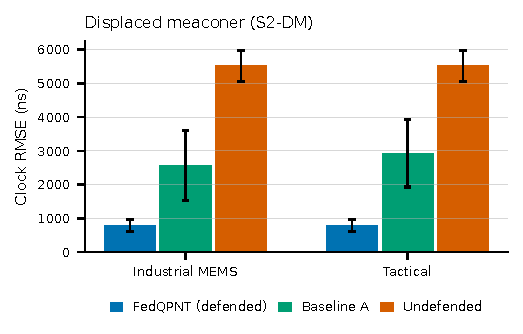
\includegraphics[width=\columnwidth]{figures/results_timing_meaconing.pdf}
\caption{Clock error under the displaced meaconer: mean and 95\% CI over 30 seeds, for both IMU grades.}
\label{fig:clock}
\end{figure}

Trust was also stable. The largest number of trust cycles in any run was 29 per hour, well inside the 223 bound. Over the four-hour run, the ratio of last-hour to first-hour error was 0.79 (MEMS) and 0.84 (tactical), and the covariance stayed positive definite.

\subsection{Where it does not}
Under small and medium drift spoofs, FedQPNT was worse than doing nothing (Table~\ref{tab:head}, Fig.~\ref{fig:dvu}). The reason is simple once seen. A spoof that drags the solution by tens of metres per minute does less damage than several minutes of MEMS coasting. Excluding GNSS is only worthwhile when the attacker's displacement exceeds the inertial drift over the exclusion period, and our engine does not yet check this. Recovery after the meaconer was also slower than Baseline A's (median post-attack error 1{,}310\,m against 268\,m), because FedQPNT waits for its next probe. That is the price of refusing memoryless re-admission. Finally, when the true receiver noise was at least twice what the receiver reported, the evidence tests fired continuously and GNSS was locked out on clean data.

\begin{figure}[t]
\centering
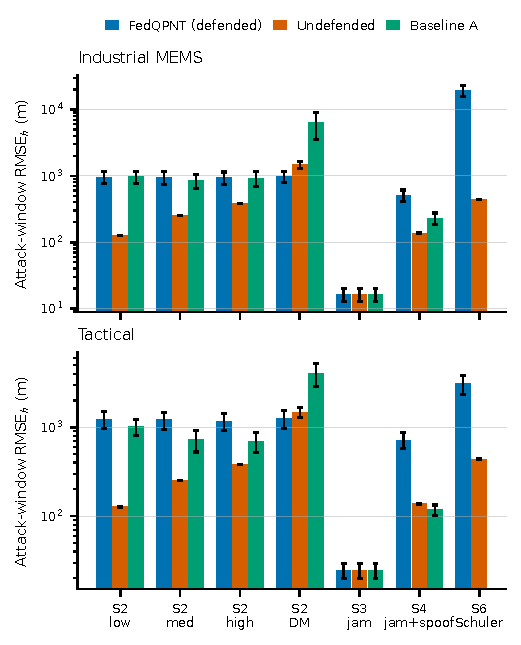
\includegraphics[width=\columnwidth]{figures/results_defended_vs_undefended.pdf}
\caption{Attack-window horizontal RMSE per scenario (mean and 95\% CI over 30 seeds, log scale) for FedQPNT, the undefended filter and Baseline A.}
\label{fig:dvu}
\end{figure}

\section{Discussion}

The results suggest that, at least in this setup, the value of a trust engine lies less in detecting attacks than in deciding what to do once they are detected. Separate clock trust gave the largest single effect we measured, and it costs almost nothing to implement. The shadow probe stopped the failure that hurt Baseline A in the meaconer case, where an early re-admission let the attacker pull the solution kilometres away. The same caution makes recovery slower and turns small spoofs into a net loss. Both problems point to the same remedy: make the exclusion decision and the dwell time depend on the predicted coast drift relative to the estimated spoof displacement.

The two null results deserve a direct statement. The CAI did not help because its contrast is lost in ordinary turns and, during straight coasts, attitude errors dominated the error budget. The federated detector did not help because the attack used for that test produced almost no feature signature. Neither result says that these components cannot help. They say that, in this configuration, we could not measure a benefit.

All results are from simulation. Attacks, sensors and the CAI are modelled on published measurements, but tests with a licensed GNSS signal simulator and real receivers are still needed.

\section{Conclusion}

We have presented a GNSS trust engine that refuses to re-admit a signal until it has been checked against an independent coast, keeps separate trust for position and timing, and uses a covariance model that keeps that check meaningful. In a pre-registered study of 5{,}340 simulated runs, it detected attacks faster than detect-and-exclude, added no cost in benign conditions, and reduced timing error under meaconing about eightfold. It also lost to an undefended receiver under small spoofs. Next steps are an adaptive dwell time, exclusion only when it is predicted to pay, and hardware-in-the-loop trials.

\section*{Acknowledgment}
The authors thank d'Armagnac de Castanet et al.\ for releasing the atom-interferometer dataset under CC-BY-4.0.
% If AI tools were used in preparing this manuscript, disclose here as the venue's policy requires.

\bibliographystyle{IEEEtran}
\bibliography{refs}

\end{document}
